%% abtex2-modelo-include-comandos.tex, v-1.9.5 laurocesar
%% Copyright 2012-2015 by abnTeX2 group at http://www.abntex.net.br/ 
%%
%% This work may be distributed and/or modified under the
%% conditions of the LaTeX Project Public License, either version 1.3
%% of this license or (at your option) any later version.
%% The latest version of this license is in
%%   http://www.latex-project.org/lppl.txt
%% and version 1.3 or later is part of all distributions of LaTeX
%% version 2005/12/01 or later.
%%
%% This work has the LPPL maintenance status `maintained'.
%% 
%% The Current Maintainer of this work is the abnTeX2 team, led
%% by Lauro César Araujo. Further information are available on 
%% http://www.abntex.net.br/
%%
%% This work consists of the files abntex2-modelo-include-comandos.tex
%% and abntex2-modelo-img-marca.pdf
%%

% ---
% Este capítulo, utilizado por diferentes exemplos do abnTeX2, ilustra o uso de
% comandos do abnTeX2 e de LaTeX.
% ---
 
\chapter{Background}\label{background}
\chapterprecis{The purpose of this section is to understand the problem.}\index{sinopse de capítulo}

% ---
\section{Similar Selection Systems}
% ---

\noindent
An optimization procedure which is similar to ours is presented by \cite{raynersss13}, but their procedure maximizes the average heuristic value. By contrast, the meta$-$reasoning we are proposing minimizes the search tree size.\\

Our meta$-$reasoning requires a prediction of the number of nodes expanded by A$\sp{*}$ using any given subset. Although there are methods for accurately predicting the number of nodes expanded by Iterative Deepening$-$A$\sp{*}$ \cite{Korf85ida} (ID$A\sp{*}$). (\texttt{SS} system  \cite{lelis2013predicting}), these methods can't be easily adapted to A$\sp{*}$ because A$\sp{*}$'s duplicate pruning makes it very difficult to predict how many nodes will occur at depth $d$ of $A\sp{*}$'s search tree (the tree of nodes expanded by $A\sp{*}$). As a part of our proposal, we present \texttt{SS} for predicting the size of the search tree.

The system most similar to ours is \textbf{RIDA$\sp{*}$} \cite{BarleySantiagoOver}. \textbf{RIDA$\sp{*}$} also selects a subset from a pool of heuristics to guide the $A\sp{*}$ search. In \textbf{RIDA$\sp{*}$} this is done by starting with an empty subset and trying all combination of size one before trying the combination of size two and so on. \textbf{RIDA$\sp{*}$} stops after evaluating a fixed number of subsets. While \textbf{RIDA$\sp{*}$} is able to evaluate a set of heuristics with tens of elements, our meta$-$reasoning is able to evaluate a set of heuristics with thousands of elements.

% ---
\section{Problem definition}
% ---

A $SAS\sp{+} planning\ task$ \cite{backstrom1995complexity} is a 4 tuple $\triangledown = \{V, O, I, G\}.$ \textit{V} is a set of \textit{state variables.} Each variable \textit{v} $\in$ \textit{V} is associated with a finite domain of possible $D_{\substack{v}}$. A state is an assignment of a value to every $v \in V.$ The set of possible states, denoted \textit{V}, is therefore $D_{\substack{v_{\substack{1}}}}    \times ... \times D_{\substack{v_{\substack{2}}}}$. \textit{O} is a set of operators, where each operator $o \in O$ is triple $\{pre_{\substack{o}} , post_{\substack{o}}, cost_{\substack{o}}\}$ specifying the preconditions, postconditions (effects), and non-negative cost of \textit{o}. $pre_{\substack{o}}\ and\ post_{\substack{o}}$ are assignments of values to subsets os variables, $V_{\substack{pre_{\substack{o}}}}\ and\ V_{\substack{post_{\substack{o}}}}$, respectively. Operator \textit{o} is applicable to state \textit{s} if \textit{s} and $pre_{\substack{o}}$ agree on the assignment of values to variables in $V_{\substack{pre_{\substack{o}}}}$. The effect of \textit{o}, when applied to \textit{s}, is to set the variables in $V_{\substack{post_{\substack{o}}}}$ to the values specified in $post_{\substack{o}}$ and to set all other variables to the value they have in \textit{s}. \textit{G} is the goal condition, an assignment of values to a subset of variables, $V_{\substack{G}}$. A state is a goal state if it and \textit{G} agree on the assignment of values to the variable in $V_{\substack{G}}$. \textit{I} is the initial state, and the planning task, $\triangledown$, is to find an optimal (least-cost) sequence of operators leading from \textit{I} to a goal state. We denote the optimal solution cost of $\triangledown$ as $C\sp{*}$ \\

The state space problem illustrated in the figure \ref{fig:8tilepuzzle_begin} is a game that consists of a frame of numbered square tiles in random order with one tile missing. The puzzle also exists in other sizes, particularly the smaller 8$-$puzzle. If the size is 3$\times$3 tiles, the puzzle is called the 8$-$puzzle or 9$-$puzzle, and if 4 $\times$ 4 tiles, the puzzle is called the 15$-$puzzle or 16$-$puzzle named, respectively, for the number of tiles and the number of spaces. The object of the puzzle is to place the tiles in order by making sliding moves that use the empty space. \\

The legal operators are to slide any tile that is horizontally or vertically adjacent to the blank into the blank position. The problem is to rearrange the tiles from some random initial configuration into a particular desired goal configuration. The 8$-$puzzle contains 181,440 reachable states, the 15$-$puzzle contains about $10\sp{13}$ reachable states, and the 24$-$puzzle contains almost $10\sp{25}$ states. \\

\begin{figure}[htb]
\centering
\begin{forest}
 [\usebox\myboxa \hspace*{1.4in} \usebox\myboxb]
 $\node [xshift=-5.5cm,yshift=3.5cm] (A) at (2,0) {Initial};$
 $\node [xshift=1.5cm,yshift=3.5cm] (A) at (2,0) {Goal};$
\end{forest}
\caption{The left tile$-$puzzle is the initial distribution of tiles and the right tile$-$puzzle is the goal distribution of tiles. Each one represent a State.} \label{fig:8tilepuzzle_begin}
\end{figure}


Instead of using an algorithm of Brute force search that will analyze all the possible solutions. We can obtain heuristics from the problem of the slide tile puzzle that will help us to solve the problem.

\section{Heuristics}
State$-$space algorithms, such as A* \cite{hart1968formal}, are important in many \texttt{AI} applications. A* uses the $f(s) = g(s) + h(s)$ cost function to guide its search. Here, $g(s)$ is the cost of the path from the start state $s$, and $h(s)$ is the estimated cost$-$to$-$go from $s$ to a gial; $h(.)$ is known as the heuristic function. The heuristic is the mathematical concept that represent to the estimate distance from the node $s$ to the nearest goal state.

\begin{figure}[htb]
\centering
\begin{tikzpicture}
	%\draw[yshift=-1 em, ultra thick] (0,0) [point] -- (5,0) [point] -- (10,0) [point];
	\coordinate (I) at (0,0) (I) node[point=ultra thick, above] {I};
	\coordinate (I1) at (2,0) (I1) node[point=ultra thick, above] {};
	\coordinate (I2) at (4,0) (I2) node[point=ultra thick, above] {};
	\coordinate (I3) at (6,0) (I3) node[point=ultra thick, above] {};
	\coordinate (s) at (8,0) (s) node[point=ultra thick, above] {s};
	\coordinate (I4) at (10,0) (I4) node[point=ultra thick, above] {};
	\coordinate (I5) at (12,0) (I5) node[point=ultra thick, above] {};
	\coordinate (G) at (14,0) (G) node[point=ultra thick, above] {G};
	\draw (I) -- (G);	

\draw [decorate,decoration={brace,amplitude=4pt},xshift=4pt,yshift=14pt]
(8,0) -- (12,0) node [black,midway,yshift=0.5cm] 
{\footnotesize $h(s)=2$};

\draw [decorate,decoration={brace,amplitude=8pt,mirror},xshift=4pt,yshift=-14pt]
(0,0) -- (8,0) node [black,midway,yshift=-0.5cm] 
{\footnotesize $g(s)=4$};


\draw [decorate,decoration={brace,amplitude=6pt,mirror},xshift=4pt,yshift=-14pt]
(8,0) -- (14,0) node [black,midway,yshift=-0.5cm] 
{\footnotesize $h\sp{*}(s)=3$};
\end{tikzpicture}
\caption{Heuristic Search: \textit{I}: Initial State, \textit{s}: Some Sate, \textit{G}: Goal State} \label{fig:searchSpace}
\end{figure}

In the figure \ref{fig:searchSpace} the optimal distance from the Initial State $I$ to  the state $s$ is 4 and represented by $g(s)$. The $h\sp{*}(s)$ represent the optimal distance from $s$ to the Goal State $G$. And the $h(s)$ is the estimation distance from $s$ to $G$.

A heuristic function $h(s)$ estimates the cost of a solution path from $s$ to a goal state. A heuristic is admissible if $h(s) \leq h\sp{*}(s)$ for all $s \in V$, where $h\sp{*}(s)$ is the optimal cost of $s$. A heuristic is consisten iff $h(s) \leq c(s,t) + h(t)$ for all states $s$ and $t$, where $c(s,t)$ is the cost of the cheapest path from $s$ to $t$. For example, the heuristic function provided by a pattern database (\texttt{PDB}) heuristic \cite{culberson1998pattern} is admissible and consistent.

Given a set of admissible and consistent heuristics $\zeta = \{h_{1}, h_{2}, \dots, h_{M}\}$, the heuristic $h_{max}(s,\zeta) = $max$_{h \in \zeta} h(s)$ is also admissible and consistent. When describing our method we assume all heuristics to be consistent. We define $f_{max}(s, \zeta) = g(s) + h_{max}(s, \zeta)$, where $g(s)$ is the cost of the path expanded from $I$ to $s$. $g(s)$ is minimal when A$\sp{*}$ using a consistent heuristic expands $s$. We call an A$\sp{*}$ search tree the tree defined by the states expanded by A$\sp{*}$ using a consistent heuristic while solving a problem $\triangledown$.

The heuristics can be obtained from each state of the problem. For example, for the problem of the 8$-$tile$-$puzzle figure \ref{fig:8tilepuzzle_begin} we can get two heuristics.

\subsection{Out of place (O.P)}
Counts the number of objects out of place.

\begin{figure}[htb]
\centering
\begin{forest}
 [\usebox\myboxa]
 $\draw[->,xshift=4pt,yshift=14pt] (2,1) -- (4,1);$
 $\node [xshift=1cm,yshift=2cm] (A) at (2,0) {O.P=8};$
 \hspace*{1.8in} 
 %$\rightarrow$  
 [\usebox\myboxb] 
\end{forest}
\caption{Out of place heuristic} \label{fig:8tilepuzzle_oop}
\end{figure}

The tiles numbered with 4, 1, 2, 3, 6, 7, 5, 8, and 4 are out of place then each object count as 1 and the sum would be 8.

\subsection{Manhatham Distance (M.D)}
Counts the minimum number of operations to get to the goal state.

\begin{figure}[htb]
\centering
\begin{forest}
 [\usebox\myboxa]
 $\draw[->,xshift=4pt,yshift=14pt] (2,1) -- (4,1);$
 $\node [xshift=1cm,yshift=2cm] (A) at (2,0) {M.D=1O};$
 \hspace*{1.8in} 
 %$\rightarrow$  
 [\usebox\myboxb] 
\end{forest}
\caption{Manhatham distance heuristic} \label{fig:8tilepuzzle_md}
\end{figure}

The tile 4 count 1 to get to the goal position.
The tile 1 count 1 to get to the goal position.
The tile 2 count 1 to get to the goal position.
The tile 3 count 1 to get to the goal position.
The tile 6 count 1 to get to the goal position.
The tile 7 count 1 to get to the goal position.
The tile 5 count 1 to get to the goal position.
The tile 8 count 1 to get to the goal position.
Then the sum would be 10.

In order to solve the problem, we get the heuristics, which are information from the problem to solve the problem. Exists systems that can create heuristics for each problem. Those systems are called Heuristic Generators.

\section{Heuristic Generators}
Heuristic Generators works by creating abstractions of the original problem space. The approach that has showed more successful results lately is \texttt{PDB}.

\subsection{Pattern Database (PDB)}
It's obtained by abstracting away certain problem variables, so that the remaining problem ("pattern") is small enough to be solved optimally for every state by blind exhaustive search. The results stored in a table, represent a PDB for the original problem. The abstraction of the search space gives an admissible heuristic function, mapping states to lower bounds.

\section{Take advantage of Heuristics}
The heuristics generators can create hundreds or even thousand of heuristics. In fact, exists different ways to take advantage of those heuristics. For example: If we want to use all the heuristics created by the heuristic generator. It would not be a good idea to use all of them because the main problem involved would be the time to evaluate each heuristic in the search tree, it could take too much time. \\

One way to take advantage of heuristics would be to take the maximum of the set of heuristics. For example, using three different heuristics $h1, h2$ and max($h1, h2$). Heuristic $h1$ and $h2$ are based on domain abstractions and the max($h1, h2$) is the maximum heuristic value of $h1$ and $h2$. \\

Exists different approaches to take advantage from a large set of heuristics. In this dissertation we use the meta$-$reasoning based on the minimum evaluation time. \\


\section{Number of heuristics created}
Let's suppose we have to run our meta$-$reasoning using M amount of memory available. The question would be: How many heuristics our system should handle in order to avoid out of memory errors? So. one of the objectives of this tesis is to find the number of heuristics that our subset $\zeta\sp{'}$ should have.

\begin{figure}[htb]
  \centering
  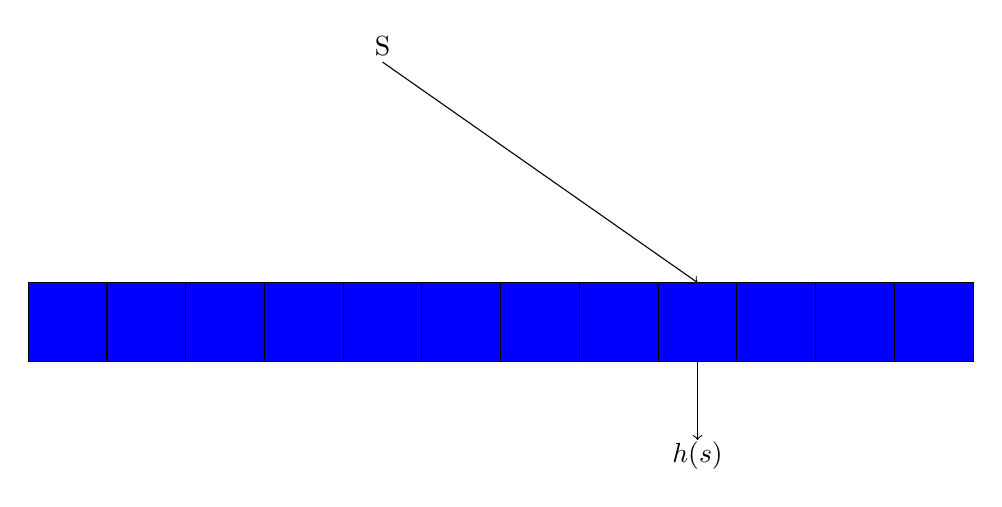
\begin{tikzpicture}
\draw[step=1cm,gray,very thin] grid (12,1);
%\draw[step=1cm,gray,very thin] (-1.9,-1.9) grid (5.9,5.9);
%\fill[blue!40!white] (0,0) rectangle (4,4);
\filldraw[fill=blue, draw=black] rectangle (12,1);
\filldraw[fill=blue, draw=black] rectangle (11,1);
\filldraw[fill=blue, draw=black] rectangle (10,1);
\filldraw[fill=blue, draw=black] rectangle (9,1);
\filldraw[fill=blue, draw=black] rectangle (8,1);
\filldraw[fill=blue, draw=black] rectangle (7,1);
\filldraw[fill=blue, draw=black] rectangle (6,1);
\filldraw[fill=blue, draw=black] rectangle (5,1);
\filldraw[fill=blue, draw=black] rectangle (4,1);
\filldraw[fill=blue, draw=black] rectangle (3,1);
\filldraw[fill=blue, draw=black] rectangle (2,1);
\filldraw[fill=blue, draw=black] rectangle (1,1);

 %$\draw[->,xshift=4pt,yshift=14pt] (2,1) -- (4,1);$
 \node [xshift=2.5cm,yshift=4cm] (A) at (2,0) {S};
 
 %\draw[->] (2.5cm,8em) -- (8cm,5em) node[midway,right] {\Om{2}};
 \draw[->] (4.5,3.8) -- (8.5,1) node[midway,right] {\Vpi{}};
 \draw[->] (8.5,0) -- (8.5,-1) node[xshift=0cm,yshift=-0.2cm] {$h(s)$};
\end{tikzpicture}
  \caption{One heuristic of size M}\label{fig:image1mem}
\end{figure}

\begin{figure}[htb]
  \centering
  \begin{tikzpicture}
\draw[step=1cm,gray,very thin] grid (12,1);
%\draw[step=1cm,gray,very thin] (-1.9,-1.9) grid (5.9,5.9);
%\fill[blue!40!white] (0,0) rectangle (4,4);
\filldraw[fill=green, draw=black] rectangle (12,1);
\filldraw[fill=green, draw=black] rectangle (11,1);
\filldraw[fill=green, draw=black] rectangle (10,1);
\filldraw[fill=green, draw=black] rectangle (9,1);
\filldraw[fill=green, draw=black] rectangle (8,1);
\filldraw[fill=green, draw=black] rectangle (7,1);
\filldraw[fill=blue, draw=black] rectangle (6,1);
\filldraw[fill=blue, draw=black] rectangle (5,1);
\filldraw[fill=blue, draw=black] rectangle (4,1);
\filldraw[fill=blue, draw=black] rectangle (3,1);
\filldraw[fill=blue, draw=black] rectangle (2,1);
\filldraw[fill=blue, draw=black] rectangle (1,1);

 %$\draw[->,xshift=4pt,yshift=14pt] (2,1) -- (4,1);$
 \node [xshift=2.5cm,yshift=4cm] (A) at (2,0) {S};
 
 %\draw[->] (2.5cm,8em) -- (8cm,5em) node[midway,right] {\Om{2}};
 \draw[->] (4.5,3.8) -- (4.5,1) node[midway,right] {\Vpi{1}};
 \draw[->] (4.5,0) -- (4.5,-1) node[xshift=0cm,yshift=-0.2cm] {$h_{\substack{1}}(s)$};
 
 \draw[->] (4.5,3.8) -- (8.5,1) node[midway,right] {\Vpi{2}};
 \draw[->] (8.5,0) -- (8.5,-1) node[xshift=0cm,yshift=-0.2cm] {$h_{\substack{2}}(s)$};
 
 \draw[decorate,decoration={brace,amplitude=8pt,mirror},xshift=4pt,yshift=-1.5cm]
(4,0) -- (9,0) node [black,midway,yshift=-0.5cm] 
{\footnotesize $max$};
\end{tikzpicture}
  \caption{Two heuristics of size M/2}\label{fig:image2mem}
\end{figure}

\begin{figure}[htb]
  \centering
  \begin{tikzpicture}
\draw[step=1cm,gray,very thin] grid (12,1);
%\draw[step=1cm,gray,very thin] (-1.9,-1.9) grid (5.9,5.9);
%\fill[blue!40!white] (0,0) rectangle (4,4);
\filldraw[fill=blue, draw=black] rectangle (12,1);
\filldraw[fill=blue, draw=black] rectangle (11,1);
\filldraw[fill=orange, draw=black] rectangle (10,1);
\filldraw[fill=orange, draw=black] rectangle (9,1);
\filldraw[fill=red, draw=black] rectangle (8,1);
\filldraw[fill=red, draw=black] rectangle (7,1);
\filldraw[fill=brown, draw=black] rectangle (6,1);
\filldraw[fill=brown, draw=black] rectangle (5,1);
\filldraw[fill=yellow, draw=black] rectangle (4,1);
\filldraw[fill=yellow, draw=black] rectangle (3,1);
\filldraw[fill=green, draw=black] rectangle (2,1);
\filldraw[fill=green, draw=black] rectangle (1,1);

 %$\draw[->,xshift=4pt,yshift=14pt] (2,1) -- (4,1);$
 \node [xshift=2.5cm,yshift=4cm] (A) at (2,0) {S};

 \draw[->] (4.5,3.8) -- (1,1) node[midway,right] {\Vpi{1}};
 \draw[->] (1,0) -- (1,-1) node[xshift=0cm,yshift=-0.2cm] {$h_{\substack{1}}(s)$};
 
 \draw[->] (4.5,3.8) -- (11,1) node[midway,right] {\Vpi{n}};
 \draw[->] (11,0) -- (11,-1) node[xshift=0cm,yshift=-0.2cm] {$h_{\substack{n}}(s)$};
 
%draw each arrow
\draw[->] (3,0) -- (3,-1) node[xshift=0cm,yshift=-0.2cm] {};
\draw[->] (5,0) -- (5,-1) node[xshift=0cm,yshift=-0.2cm] {};
\draw[->] (7,0) -- (7,-1) node[xshift=0cm,yshift=-0.2cm] {};
\draw[->] (9,0) -- (9,-1) node[xshift=0cm,yshift=-0.2cm] {}; 

 \draw[decorate,decoration={brace,amplitude=12pt,mirror},xshift=4pt,yshift=-1.5cm]
(0,0) -- (12,0) node [black,midway,yshift=-0.7cm] 
{\footnotesize $max$};
\end{tikzpicture}
  \caption{N heuristics of size M/N}\label{fig:image3mem}
\end{figure}

In the Figures \ref{fig:image2mem} and \ref{fig:image3mem} we are taking advantange of the heuristics doing the maximization of all the heuristics created.

\clearpage

\section{Heuristic Subset}
The heuristics generator systems can create a large number of heuristics. Let's suppose $|\zeta| = $ 1000 heuristics were created considering the time and memory avaiable and we want to select the best N $=$ 100 heuristics. This would be: $${1000\choose 100} = 10\sp{138} possibilities$$
So, try to select heuristics from a large set of heuristics are going to be treated as an optimization problem. Then, in order to obtain a good selection of subset of heuristics, our objective function should guarantee two properties: Monotonicity and Submodularity, that would be explained in the next Part. \\
 \bigskip

In the next Part, we will introduce the meta$-$reasoning proposed for selecting heuristics and will expand on the properties of our objective functions.\\


\section{Problem Domains}
The problems we are trying to solve are the optimal domains for International Planning Competition (\texttt{IPC}).

\subsection{Blocks world}
This domain consists of a set of blocks, a table and a robot hand. The blocks can be on top of other blocks or on the table; a block that has nothing on it is clear; and the robot hand can hold one block or be empty. The goal is to find a plan to move from one configuration of blocks to another.

\begin{figure}[htb]
\centering
\begin{forest}
[\usebox\myboxblockteststar \hspace*{0.2in} \usebox\myboxblockredthree \hspace*{1.5in} \usebox\myboxblocktestend]
\end{forest}
\caption{Blocks world with three blocks.}\label{fig:probblocks}
\end{figure}

The solution shown in Figure \ref{fig:probblocks} is to unblock number 1 from block number 2; stack block number 2 on block number 1; finally, stack blocl number 3 on block number 2. We are interestred in optimal or near$-$optimal solutions for this kind of problem.\\

Depending on the number $n$ of blocks this domain can have very large state spaces. For example, using $n = 20$ this domain has approximately $10\sp{20}$ different states.


\subsection{Barman}



\clearpage